\chapter{Speaker Recognition Systems}
\label{ch:speaker-recognition-systems}

%TODO remodelar, retirando tudo sobre Speaker IDENTIFICATION

The speaker recognition process lies on the field of pattern classification, with the speaker's speech signal $\boldsymbol{Y}$ as input for a classifier. For an identification system, the classification is 1 to N (one speaker signal to be identified as belonging to one of the N enrolled speakers), while for a verification system the classification is 1 to 1 (a claimed speaker identity is \emph{enrolled} or \emph{imposter}).

Automatic Speaker Recognition (ASR) systems are bayesian classifiers, using the following equation to calculate the probabilities of recognition:

\begin{equation}
    \postprob{\mathcal{S}}{\boldsymbol{Y}} = \frac{\postpdf{\boldsymbol{Y}}{\mathcal{S}} \prob{\mathcal{S}}}{\pdf{\boldsymbol{Y}}},
    \label{eq:bayes_equation}
\end{equation}

\noindent where $\mathcal{S}$ is the speaker who produced $\boldsymbol{Y}$. As all speakers are considered equally probable, the \emph{a priori} probability $\prob{\mathcal{S}}$ and the \emph{evidence} $\pdf{\boldsymbol{Y}}$ (just used for normalization) can be removed with no loss to the analysis. \equationref{bayes_equation} is then replaced by $\postpdf{\boldsymbol{Y}}{\mathcal{S}}$.

\section{Basic Concepts}
\label{sec:basic-concepts}

Before start the discussion about the types of ASR systems, some basic concepts must be elucidated. Those are \textbf{utterance} and \textbf{features}.

\subsection{Utterance}

An utterance is a piece of speech produced by a speaker. It may be a word, a statement or any vocal sound. The terms \emph{utterance} and \emph{speech signal} sometimes are used interchangeably, but from herenow speech signal will be defined as an utterance recorded, digitalized and ready to be processed. An example is shown in \figureref{speech_signal}.

\begin{figure}[ht]
    \centering
    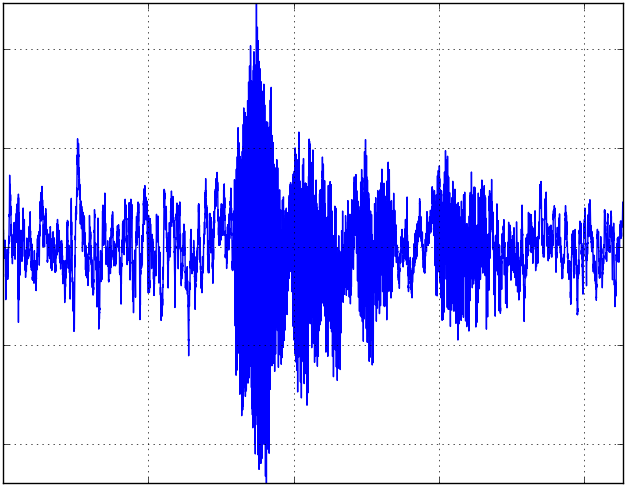
\includegraphics[width=\textwidth]{chapters/speaker-recognition-systems/speech_signal}
    \caption{Speech signal from utterance ``karen livescu", \refbib{Woo, Park \& Hazen}{woo.park.hazen.2006}.}
    \label{fig:speech_signal}
\end{figure}

\subsection{Features}

The raw speech signal is unfit for use by an ASR system. For a correct processing, the representative features from the speaker's vocal tract are extracted, what reduces the number of variables the system needs to deal with (leading to a simpler implementation) and performs a better evaluation (prevents the curse of dimensionality). Due to the stationary properties of the speech signal when analyzed in a short period of time, it is divided in overlapping frames of small and predefined length, to avoid ``loss of significance", \refbib{Davis \& Mermelstein}{davis.mermelstein.1980}, \refbib{Rabiner \& Schafer}{rabiner.schafer.2007}. This extraction is executed by the MFCC algorithm, explained in details in \chapterref{feature-extraction}.

\section{Speaker Identification}
\label{sec:speaker-identification}

Given a sequence $\dvec{X}$ of features extracted from a speech signal $\dvec{Y}$ spoken by an arbitrary speaker $\mathcal{S}$, the task of identify $\mathcal{S}$ as a particular $\mathcal{S}_i$ from $\dvec{\mathcal{S}}$ (set of enrolled users) is given by the following equation:

\begin{equation}
    \mathcal{S} \text{ is } \mathcal{S}_i \text{ if } i = \arg_j\max\postpdf{\boldsymbol{X}}{\mathcal{S}_j},
    \label{eq:classification_speaker_identification}
\end{equation}

\noindent for $j = 1, ..., S$ (where $S$ is the size of $\dvec{\mathcal{S}}$). The high level speech $\boldsymbol{Y}$ in $\postpdf{\boldsymbol{Y}}{\mathcal{S}}$ is replaced by $\boldsymbol{X}$ in \equationref{classification_speaker_identification}, a proper way to represent the signal's characteristics.

\subsection{Training}

The features extracted from speech signals are used to train models for the speakers. Each speaker $\mathcal{S}_j$ is represented by a model $\lambda_j$, generated using only features from the speaker.

\begin{figure}[ht]
    \centering
    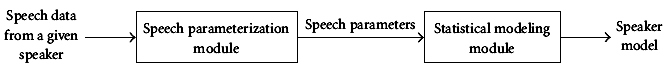
\includegraphics[width=\textwidth]{chapters/speaker-recognition-systems/speaker-recognition-training}
    \caption{The statistical model of $\mathcal{S}$ is created from the speech signal $\dvec{Y}$, \refbib{Bimbot et. al.}{bimbot.et.al.2004}.}
    \label{fig:speaker-recognition-training}
\end{figure}

The idea behind the training stage is to make $\lambda_j$ ``memorize" the distinct characteristics present in the speaker's vocal tract that perform the identification. The SSGMM, initially referenced in \sectionref{gmm} and described in details in \chapterref{gmm}, is a perfect choice to model the $\lambda_j$'s.

\subsection{Test}

The system test is performed replacing $\mathcal{S}_j$ in \equationref{classification_speaker_identification} by the model $\lambda_j$, leading to

\begin{equation}
    \mathcal{S} \text{ is } \mathcal{S}_i \text{ if } i = \arg_j\max\postpdf{\boldsymbol{X}}{\lambda_j},
    \label{eq:speaker_identification}
\end{equation}

\noindent where the $\lambda_j$ with higher probability has its identity assigned to $\mathcal{S}$. The main difficult this system presents is the fact that every $\dvec{X}$ must be tested with every $\mathcal{S}_j$ from $\dvec{\mathcal{S}}$, as seen in \figureref{speaker_identification}, what demands a high amount of time.

\begin{figure}[ht]
    \centering
    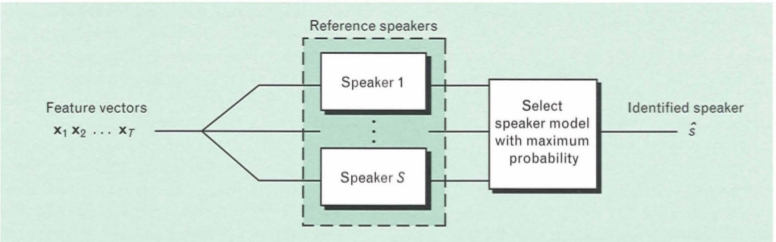
\includegraphics[width=\textwidth]{chapters/speaker-recognition-systems/speaker-identification}
    \caption{Speaker identification test, \refbib{Reynolds}{reynolds.1995a}.}
    \label{fig:speaker_identification}
\end{figure}

\section{Speaker Verification}
\label{sec:speaker-verification}

If a speaker $\mathcal{S}$ claims to be a particular user $\mathcal{S}_i$ from $\dvec{\mathcal{S}}$, the strength of this claim resides on how similar the features $\dvec{X}$ are to the features from $\mathcal{S}_i$ ``memorized" by the system. Then a simple equation

\begin{equation}
    \postpdf{\boldsymbol{X}}{\mathcal{S}_i} \verifytestB{\alpha}{\mathcal{S}}
    \label{eq:decision_speaker_verification}
\end{equation}

\noindent where $\alpha$ is an arbitrary coefficient, should be enough (considering all speakers equally probable). However, a subset of enrolled speakers may have vocal similarities or the features $\dvec{X}$ may be common to a large number of users, leading to a misclassification of an imposter as a registered speaker (a false detection). To reduce the error rate, the system must decide not only if a speech signal came from the claimed speaker, but also if it came from a set composed of all other enrolled speakers and compare the likelihoods.

\subsection{Likelihood Ratio Test}

Given the vector of features $\dvec{X}$, and assuming it was produced by only one speaker, the detection\footnote{the terms verification and detection are used interchangeably} task can be restated as a basic test between two hypoteses, \refbib{Reynolds}{reynolds.1995b}:

\begin{description}\itemsep0pt
    \item $H_0$: $\dvec{X}$ is from the claimed speaker $\mathcal{S}_i$;
    \item $H_1$: $\dvec{X}$ is \underline{not} from the claimed speaker $\mathcal{S}_i$.
\end{description}

\noindent The optimum test to decide which hypotesis is valid is the \textbf{likelihood ratio test} between both likelihoods $\postpdf{\dvec{X}}{H_0}$ and $\postpdf{\dvec{X}}{H_1}$, \refbib{Reynolds, Quatieri \& Dunn}{reynolds.quatieri.dunn.2000},

\begin{equation}
    \frac{\postpdf{\dvec{X}}{H_0}}{\postpdf{\dvec{X}}{H_1}} \verifytestB{\theta}{H_0}
    \label{eq:likelihood-ratio-test}
\end{equation}

\noindent where the decision threshold for accepting or rejecting $H_0$ is $\theta$ (a low $\theta$ generates a more permissive system, while a high $\theta$, a more restrictive). Applying the logarithm, the behavior of the likelihood ratio is maintained and \equationref{likelihood-ratio-test} is replaced by the \textbf{log-likelihood ratio}

\begin{equation}
    \Lambda(\dvec{X}) = \log \postpdf{\dvec{X}}{H_0} - \log \postpdf{\dvec{X}}{H_1}.
    \label{eq:log-likelihood-ratio-test}
\end{equation}

\subsection{Training}

Once the features are extracted from the speech signal, they are used to train the models $\lambda_{hyp}$ and $\lambda_{\overline{hyp}}$ for $H_0$ and $H_1$, respectively. A high-level demonstration of the training of $\lambda_{hyp}$ (mathematical representation of $\mathcal{S}_i$) is shown in \figureref{speaker-recognition-training}.

Due to $\lambda_{hyp}$ be a model of $\mathcal{S}_i$, the features used for training (i.e., estimate $p(\dvec{X}|\lambda_{hyp})$) are extracted from speech signals produced by $\mathcal{S}_i$. The model $\lambda_{\overline{hyp}}$, however, is not well-defined. It should be composed of the features extracted from speech signals from all other speakers except $\mathcal{S}_i$, but creating a single $\lambda_{\overline{hyp}}$ for each speaker is complicated and with no expressive gain. Instead, what is normally done is use all speakers to generate a background model $\lambda_{bkg}$, \refbib{Reynolds}{reynolds.1997}, in which the weights of all $\mathcal{S}_i$ are approximately equal.

\subsection{Test}

As seen in \equationref{log-likelihood-ratio-test}, the decision process is based on a function \emph{Score}. Replacing each $H_j$ for its corresponding model, the likelihood of a $\lambda_j$ given $\dvec{X} = \{\dvec{x}_1, \dots, \dvec{x}_T\}$ can be written as

\begin{equation}
    p(\dvec{X}|\lambda_j) = \prod_{t=1}^T p(\dvec{x}_t|\lambda_j).
    \label{eq:likelihood-prod}
\end{equation}

\noindent Using the logarithm function, \equationref{likelihood-prod} becomes

\begin{equation}
    \log p(\dvec{X}|\lambda_j) = \frac{1}{T} \sum_{t=1}^T \log p(\dvec{x}_t|\lambda_j),
    \label{eq:log-likelihood-sum}
\end{equation}

\noindent where the term $\frac{1}{T}$ is added to normalize the log-likelihood to the duration of the speech signal. That said, the likelihood ratio given by \equationref{log-likelihood-ratio-test} becomes

\begin{equation}
    \Lambda(\dvec{X}) = \log p(\dvec{X}|\lambda_{hyp}) - \log p(\dvec{X}|\lambda_{bkg}),
    \label{eq:score_of_X}
\end{equation}

\noindent and the speaker is accepted if $\Lambda(\dvec{X}) \geq \Theta$, for an arbitrary value of $\theta$, with $\Theta = \log\theta$ (see \figureref{speaker-verification}).

\begin{figure}[ht]
    \centering
    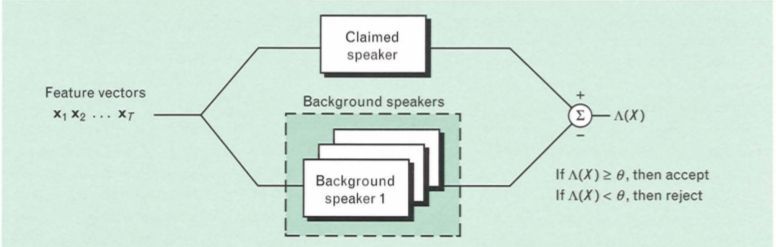
\includegraphics[width=\textwidth]{chapters/speaker-recognition-systems/speaker-verification}
    \caption{Likelihood-ratio-based speaker verification test, \refbib{Bimbot et. al.}{bimbot.et.al.2004}.}
    \label{fig:speaker-verification}
\end{figure}